In this part of my thesis, I report the results from my experiments. Since there are no direct benchmarks it's important to know how to view the results. In the simplest form, successful results can be stated when betting is profitable, which some of the models were able to achieve. Unfortunately, this is a very narrow perspective and for that reason, in this part of my thesis, I will dig deeper to see why some of the models were able to achieve profitable returns and what downsides these models and strategies might have even though they were profitable. Also, it's important to see how valuable the novel EA Sport's video game series FIFA's player attribute dataset is for the prediction.

\section{Results from tournament simulations}
Tournament simulation results for each of the models are listed in the tables \ref{table:outcomemodel}, \ref{table:scoreresults}, \ref{table:onevsrestresults} and \ref{table:linearmodel}. Tables include metrics for accuracy, log loss, unit strategy's profit, and kelly strategy's profit. Listed values are averages from 10 individual simulations and include standard deviation. All metrics are listed for every feature set used in training. Description for each feature set is listed in the table \ref{table:featuresetlist}.

First of all, it's important to see if any of the models were able to generate profit. Preferably, a model should be profitable in each of the tournaments, since investors prefer steady profits. Also, if a model is able to capture the logic from different data periods and estimate correctly based on that it's harder to say that the model was just lucky all the time.

The unit strategy is the simples strategy and for that reason, it's a good starting point. Unit strategy's profits for \textit{Outcome mode}, \textit{Score model} and \textit{OVR model} are positive in every tournament, but not with all feature sets.  Good unit profits and high accuracy go hand in hand, which is no surprise, but high accuracy is not a clear indicator for good kelly profits, which is a slight of a surprise. With kelly strategy intuition can mislead you since the only thing that matters are the probability estimate and the given odd. Too high probabilities can lead to a situation where the model with high accuracy can have too risky bets when using kelly as a betting strategy.  In fact, only \textit{Outcome model}, trained with player features, is the only model that can be profitable using both of the strategies.

Being profitable only in one out of 12 is not a great start. And since there are no direct benchmark it's even harder to say how good the performance is. Bookmaker's odds can be used to form a comparison model. ADD CALCULATIONS. Using bookmaker's average odds their accuracy on World cup 2018 and 2014 was 56.25\% (36 games correctly predicted) and 51.56  \% (33 games correctly predicted) on 2010. Most of the models that I used are able to outperform the comparison model in accuracy. Since bookmarker's use these probabilities to compute odds,  unit strategy and kelly strategy can't be compared.

But which of the feature set and model combinations is the best? This question is tricky to answer. If being profitability in every tournament with high profit is preferred than \textit{Score model}, trained with all features, might be the right choice. Whereas highest unit profits are achieved with \textit{OVR model} trained with player features. Using only these metrics to validate if a model is good enough to be trusted in the next World cup 2022 is too risky. Being profitable in 192 games (64 per three tournaments) is a good start, but it's also important to understand how the models predict individual games to understand the total profits better.

\begin{table}
    \caption{Feature set description}
    \begin{tabular}{| c | c|}
        \hline
        Feature set's name & Description \\
        \hline
        Player features & FIFA player attributes only \\
        All Features & General features and Player features \\
        General Features & All excluding Player features \\
        \hline
    \end{tabular}
    \label{table:featuresetlist}
\end{table}

\begin{table}
    \caption{Tournament characteristics. Underdog victory is a case where the winning team has higher odds for winning then the other team.}
    \begin{tabular}{| c | c|c | c|}
        \hline
        Characteristic & \textbf{WC 2018} & \textbf{WC 2014} & \textbf{WC 2010}\\
        \hline
        Home wins & 25 & 28 & 24\\
        Draws & 14 & 13 & 16\\
        Away wins & 25 & 23 & 24\\
        Underdog victory  & 14 & 15 & 14\\
        \hline
    \end{tabular}
    \label{table:tournamentcharacteristics}
\end{table}


\begin{table}
    \caption{Results for Outcome model}
    \begin{tabular}{| c  c| c| c| c|c|}
        \hline
        Metric& & \textbf{WC 2018} & \textbf{WC 2014} & \textbf{WC 2010} & Mean\\
        \hline
        Accuracy & AF & 57.34\% $\pm$ 0.72 & 60.94\% $\pm$ 1.71 & 54.84\% $\pm$ 1.09& 57.71 \\
         & GF & 52.03\% $\pm$ 1.22 & 56.56\% $\pm$ 0.62 & 55.47\% $\pm$ 1.05& 54.69 \\
         & PF & 60.47\% $\pm$ 1.41 & 59.69\% $\pm$ 0.94 & 54.22\% $\pm$ 2.22& 58.13 \\
         & & & & & \\
        Log Loss & AF & 0.9673 $\pm$ 0.0037 & 0.9362 $\pm$ 0.0047 & 0.9922 $\pm$ 0.0075& 0.9652 \\
         & GF & 1.0122 $\pm$ 0.0045 & 0.9549 $\pm$ 0.0053 & 0.9676 $\pm$ 0.0052& 0.9782 \\
         & PF & 0.9406 $\pm$ 0.0026 & 0.9503 $\pm$ 0.0024 & 1.0118 $\pm$ 0.0045& 0.9676 \\
         & & & & & \\
        Unit profit & AF & 6.39\% $\pm$ 1.96 & 15.65\% $\pm$ 5.21 & 2.93\% $\pm$ 4.43& 8.32 \\
         & GF & -3.48\% $\pm$ 3.4 & 5.17\% $\pm$ 1.52 & 5.04\% $\pm$ 3.67& 2.24 \\
         & PF & 18.38\% $\pm$ 4.26 & 12.72\% $\pm$ 2.22 & 3.32\% $\pm$ 8.33& 11.47 \\
         & & & & & \\
        Kelly profit & AF & -10.58\% $\pm$ 7.01 & 18.55\% $\pm$ 10.13 & 23.26\% $\pm$ 18.96& 10.41 \\
         & GF & -47.32\% $\pm$ 4.1 & 2.86\% $\pm$ 8.15 & 48.9\% $\pm$ 16.64& 1.48 \\
         & PF & 46.63\% $\pm$ 8.79 & 12.26\% $\pm$ 6.57 & 2.75\% $\pm$ 9.05& 20.55 \\
 \hline
    \end{tabular}
    \label{table:outcomemodel}
\end{table}


\begin{table}
    \caption{Results for Score model}
    \begin{tabular}{| c  c| c| c| c|c|}
        \hline
        Metric& & \textbf{WC 2018} & \textbf{WC 2014} & \textbf{WC 2010} & Mean\\
        \hline
        Accuracy & AF & 59.38\% $\pm$ 0.0 & 58.13\% $\pm$ 0.62 & 52.81\% $\pm$ 0.62& 56.77 \\
         & GF & 52.03\% $\pm$ 1.0 & 59.38\% $\pm$ 0.0 & 50.94\% $\pm$ 0.77& 54.12 \\
         & PF & 58.44\% $\pm$ 1.74 & 61.09\% $\pm$ 0.84 & 53.91\% $\pm$ 0.78& 57.81 \\
         & & & & & \\
        Log Loss & AF & 0.9508 $\pm$ 0.0016 & 0.935 $\pm$ 0.0005 & 0.9788 $\pm$ 0.0016& 0.9549 \\
         & GF & 0.9831 $\pm$ 0.0012 & 0.9133 $\pm$ 0.0011 & 0.9522 $\pm$ 0.001& 0.9495 \\
         & PF & 0.9566 $\pm$ 0.0013 & 0.9446 $\pm$ 0.0024 & 0.9996 $\pm$ 0.0009& 0.9669 \\
         & & & & & \\
        Unit profit & AF & 13.52\% $\pm$ 0.0 & 5.94\% $\pm$ 2.11 & -2.8\% $\pm$ 1.29& 5.55 \\
         & GF & -5.4\% $\pm$ 2.57 & 13.66\% $\pm$ 0.0 & -5.08\% $\pm$ 2.45& 1.06 \\
         & PF & 12.26\% $\pm$ 5.1 & 16.11\% $\pm$ 2.64 & 2.23\% $\pm$ 2.09& 10.2 \\
         & & & & & \\
        Kelly profit & AF & 35.59\% $\pm$ 4.45 & 12.37\% $\pm$ 1.02 & 24.2\% $\pm$ 4.43& 24.05 \\
         & GF & -19.06\% $\pm$ 1.87 & 107.61\% $\pm$ 4.47 & 99.75\% $\pm$ 3.63& 62.77 \\
         & PF & 2.04\% $\pm$ 2.62 & 10.82\% $\pm$ 4.87 & 8.3\% $\pm$ 2.1& 7.05 \\
 \hline
    \end{tabular}
    \label{table:scoreresults}
\end{table}

\begin{table}
    \caption{Results for OneVsRest model}
    \begin{tabular}{| c  c| c| c| c|c|}
        \hline
        Metric& & \textbf{WC 2018} & \textbf{WC 2014} & \textbf{WC 2010} & Mean\\
        \hline
        Accuracy & AF & 57.66\% $\pm$ 0.47 & 57.34\% $\pm$ 1.22 & 56.09\% $\pm$ 0.84& 57.03 \\
         & GF & 51.25\% $\pm$ 1.95 & 55.16\% $\pm$ 1.57 & 57.03\% $\pm$ 1.05& 54.48 \\
         & PF & 61.09\% $\pm$ 1.3 & 60.16\% $\pm$ 1.05 & 54.37\% $\pm$ 1.36& 58.54 \\
         & & & & & \\
        Log Loss & AF & 0.9646 $\pm$ 0.0035 & 0.9382 $\pm$ 0.0039 & 0.9831 $\pm$ 0.005& 0.962 \\
         & GF & 1.012 $\pm$ 0.0052 & 0.9515 $\pm$ 0.0068 & 0.9583 $\pm$ 0.0059& 0.9739 \\
         & PF & 0.9365 $\pm$ 0.0023 & 0.9564 $\pm$ 0.0032 & 1.0083 $\pm$ 0.0052& 0.9671 \\
         & & & & & \\
        Unit profit & AF & 7.31\% $\pm$ 1.04 & 5.01\% $\pm$ 2.93 & 6.52\% $\pm$ 2.97& 6.28 \\
         & GF & -5.03\% $\pm$ 4.84 & 3.04\% $\pm$ 4.31 & 10.38\% $\pm$ 3.38& 2.8 \\
         & PF & 19.83\% $\pm$ 4.01 & 14.14\% $\pm$ 2.82 & 3.88\% $\pm$ 5.11& 12.62 \\
         & & & & &  \\
        Kelly profit & AF & -2.6\% $\pm$ 6.57 & 9.34\% $\pm$ 8.69 & 26.26\% $\pm$ 10.92& 11.0 \\
         & GF & -44.81\% $\pm$ 3.96 & 14.61\% $\pm$ 13.1 & 83.44\% $\pm$ 23.89& 17.75 \\
         & PF & 61.65\% $\pm$ 9.88 & -3.92\% $\pm$ 4.68 & 0.77\% $\pm$ 7.02& 19.5 \\
 \hline
    \end{tabular}
    \label{table:onevsrestresults}
\end{table}

\begin{table}
    \caption{Results for Logistic Regression model}
    \begin{tabular}{| c  c| c| c| c|c|}
        \hline
        Metric & & \textbf{WC 2018} & \textbf{WC 2014} & \textbf{WC 2010}& Mean\\
        \hline
        Accuracy & AF & 54.84\% $\pm$ 0.84 & 63.59\% $\pm$ 0.72 & 51.41\% $\pm$ 1.3& 56.61 \\
         & GF & 51.72\% $\pm$ 1.09 & 63.28\% $\pm$ 1.26 & 54.37\% $\pm$ 1.53& 56.46 \\
         & PF & 59.69\% $\pm$ 0.62 & 62.19\% $\pm$ 0.62 & 50.78\% $\pm$ 0.78& 57.55 \\
         & & & & & \\
        Log Loss & AF & 0.9719 $\pm$ 0.0043 & 0.8791 $\pm$ 0.0025 & 1.0418 $\pm$ 0.0071& 0.9643 \\
         & GF & 0.9953 $\pm$ 0.0041 & 0.9112 $\pm$ 0.0035 & 0.9837 $\pm$ 0.0028& 0.9634 \\
         & PF & 0.9334 $\pm$ 0.0017 & 0.9311 $\pm$ 0.0032 & 1.0563 $\pm$ 0.0064& 0.9736 \\
         & & & & & \\
        Unit profit & AF & 0.79\% $\pm$ 1.51 & 27.73\% $\pm$ 3.09 & -5.11\% $\pm$ 3.88& 7.8 \\
         & GF & -3.75\% $\pm$ 2.07 & 24.57\% $\pm$ 4.51 & -0.28\% $\pm$ 5.87& 6.85 \\
         & PF & 14.73\% $\pm$ 1.93 & 21.98\% $\pm$ 2.7 & -8.95\% $\pm$ 2.03& 9.25 \\
         & & & & & \\
        Kelly profit & AF & -20.29\% $\pm$ 5.49 & 271.57\% $\pm$ 25.03 & -43.87\% $\pm$ 5.37& 69.14 \\
         & GF & -36.47\% $\pm$ 3.66 & 125.73\% $\pm$ 11.94 & 8.75\% $\pm$ 10.44& 32.67 \\
         & PF & 55.93\% $\pm$ 4.8 & 52.77\% $\pm$ 8.74 & -49.56\% $\pm$ 4.26& 19.71 \\
 \hline
    \end{tabular}
    \label{table:linearmodel}
\end{table}

\section{How models differ in game-level predictions?}
To understand the tournament simulation results better it's important to understand what happens in the game-level predictions. Analyzing all of the tournaments at game-level is out of the reach of this thesis. A single tournament can be used to see how the models differ at game-level since all of the tournaments have similar characteristics. These characteristics are listed in the table \ref{table:tournamentcharacteristics}. The only noteworthy difference is the higher number of games ending a draw in World cup 2010.

The reason why tournament with few more games ending a draw matters so much is because the models are very inaccurate when it comes to predicting the outcome of a draw. For example, the average precision of a draw for \textit{Outcome model} with any of the feature sets is at maximum 0.1. The average recall is at best 0.00625. In most of the cases, precision and recall are almost always zero. Both of those values were for World Cup 2010, meaning that only one draw from the 10 draws that were predicted in total was correct. It's no wonder that predicting draws is hard since football games often have low scores. A goal for the underdog is very valuable but not that unlikely to happen. This makes winning the game for the favorite team harder. Draws are not preferred by the bookmakers either. Very seldom draw has the lowest odds (meaning the highest probability). For example, only one game in World Cup 2010 had the lowest odds for a draw and that game didn't end a draw.

Since tournaments' characteristics are similar enough I can assume that I can use any of the tournaments to compare game-level characteristics of my models. I will use the World cup 2018 with all of the available features to compare models against each other.

I compared simulation results from all of the models for World cup 2018. Models were trained using all of the available features.

One interesting fact is that models predict outcomes are very similar - as figure \ref{fig:unit_model_comparison} shows. Outcome and score model are almost equal in their predictions. Based on the overall results models should differ more since profits are not equal or even similar. What might be the reason for this? To see more details it's wise to use the kelly strategy's cash balance progression from the figure \ref{fig:kelly_model_comparison} to compare the models. Cash balances clearly develop out of phase from the first game onward. The reason behind this is different probability distributions that the models output. By observing the tables \ref{table:home_win_metrics}, \ref{table:draw_metrics} and \ref{table:away_win_metrics} we can see that models' behaviour is fairly similar with probability prediction of a home win and an away win, but differs clearly with the prediction of a draw. Even when only random forest-based solutions are compared the difference between the models is most obvious when probability estimates for a draw are compared. The figure \ref{fig:draw_probability} shows how differently the models estimate the probability of game ending in a draw. This figure backed by the standard deviation values from the table \ref{table:draw_metrics} shows that \textit{Outcome model} and \textit{OVR model} predict probabilities of a draw more aggressively; both models sometimes predict a lot lower or higher probabilities than rest of the models. \textit{Score model} and \textit{Linear model} have significantly lower standard deviation than \textit{Outcome model} or \textit{OVR model}. Since averages from all of the models are quite close to each other this means that \textit{Score model} and \textit{Linear model} have more stable predictions. Low correlation with probability estimates with rest of the models makes \textit{linear model} the most independent. Since there are no true probabilities available for a game ending in a draw it's hard to say what is the better way to estimate the probability of a draw; is the true probability for every game closer to the average value or should the model be more flexible with the estimates. When current results are viewed less varying probability estimates for draw might be a better option since \textit{Score model} is able to make a profit with two different feature sets while \textit{Outcome model} and \textit{OVR model} are not. I compared \textit{Score model's} and \textit{Outcome model's} probability estimates to a sample probability distribution of a draw obtained from historical data. Results are in the figure \ref{fig:draw_prob_dist}.

My models predict higher probabilities for games that have a higher difference between teams' elo rating than the average is based on historical data. When sample probability distribution of a draw is taken for World Cup games only the probability line is not a as smooth, even when games are split to deciles each containing approximately 84 games. World Cup game is always important for the team, since in World Cup there are not that many opportunities to recover from bad performance. This high pressure situation can restrain even the top teams to play in a level they should be playing. These reason and a lower sample count are one of the reasons for more varying probability distribution. However eyeballing the figure \ref{fig:draw_prob_dist} indicate us that the probabilities are too high on average. This is the case even with the \textit{OVR model} as well, even though it has calibrated probability estimates.

\begin{table}[h]
    \caption{Means, standard deviations, and correlations of home win probability predictions for World cup 2018.}
    \label{table:home_win_metrics}
    \noindent
    \begin{tabular}{c c c c c c c c c c}
    \toprule
    & Measure
      & \multicolumn{1}{r}{mean}
      & \multicolumn{1}{c}{sd}
      & \multicolumn{4}{c@{}}{correlations}\\
    \cmidrule(l){5-8}
    & & & & \multicolumn{1}{c}{1{.}}
          & \multicolumn{1}{c}{2{.}}
          & \multicolumn{1}{c}{3{.}}
          & \multicolumn{1}{c@{}}{4{.}}\\
    \midrule
    & Models \\
    1{.} & Score     &   0.3956 &   0.1588 \\
    2{.} & Outcome   &   0.3854 &   0.1685 & 0.9873  \\
    3{.} & OneVsRest &   0.4016 &   0.1687 & 0.9870 &  0.9871  & \\
    4{.} & Linear    &   0.4170 & 0.1698   & 0.9654 & 0.9660   &  0.9733 \\
    \bottomrule
    \end{tabular}
    \end{table}

    \begin{table}[h]
    \caption{Means, standard deviations, and correlations of draw probability predictions for World cup 2018.}
    \label{table:draw_metrics}
    \noindent
    \begin{tabular}{c c c c c c c c c c}
    \toprule
    & Measure
      & \multicolumn{1}{r}{mean}
      & \multicolumn{1}{c}{sd}
      & \multicolumn{4}{c@{}}{correlations}\\
    \cmidrule(l){5-8}
    & & & & \multicolumn{1}{c}{1{.}}
          & \multicolumn{1}{c}{2{.}}
          & \multicolumn{1}{c}{3{.}}
          & \multicolumn{1}{c@{}}{4{.}}\\
    \midrule
    & Models \\
    1{.} & Score     &   0.2527 &   0.0274 \\
    2{.} & Outcome   &   0.2619 &   0.0414 & 0.8102  \\
    3{.} & OneVsRest &   0.2553 &   0.0414 & 0.7713  &  0.9333  & \\
    4{.} & Linear    &   0.2484 &   0.0197 & 0.2356  &  0.3162  &  0.3080 \\
    \bottomrule
    \end{tabular}
    \end{table}

    \begin{table}[h]
    \caption{Means, standard deviations, and correlations of away win probability predictions for World cup 2018.}
    \label{table:away_win_metrics}
    \noindent
    \begin{tabular}{c c c c c c c c c c}
    \toprule
    & Measure
      & \multicolumn{1}{r}{mean}
      & \multicolumn{1}{c}{sd}
      & \multicolumn{4}{c@{}}{correlations}\\
    \cmidrule(l){5-8}
    & & & & \multicolumn{1}{c}{1{.}}
          & \multicolumn{1}{c}{2{.}}
          & \multicolumn{1}{c}{3{.}}
          & \multicolumn{1}{c@{}}{4{.}}\\
    \midrule
    & Models \\
    1{.} & Score     &   0.3517 &   0.1504 \\
    2{.} & Outcome   &   0.3528 &   0.1667 & 0.9824  \\
    3{.} & OneVsRest &   0.3431 &  0.1674  & 0.9814  &  0.9889  & \\
    4{.} & Linear    &   0.3345 &  0.1753  & 0.9648  & 0.9672   &  0.9680 \\
    \bottomrule
    \end{tabular}
    \end{table}
\begin{figure}[H]
    \centering
    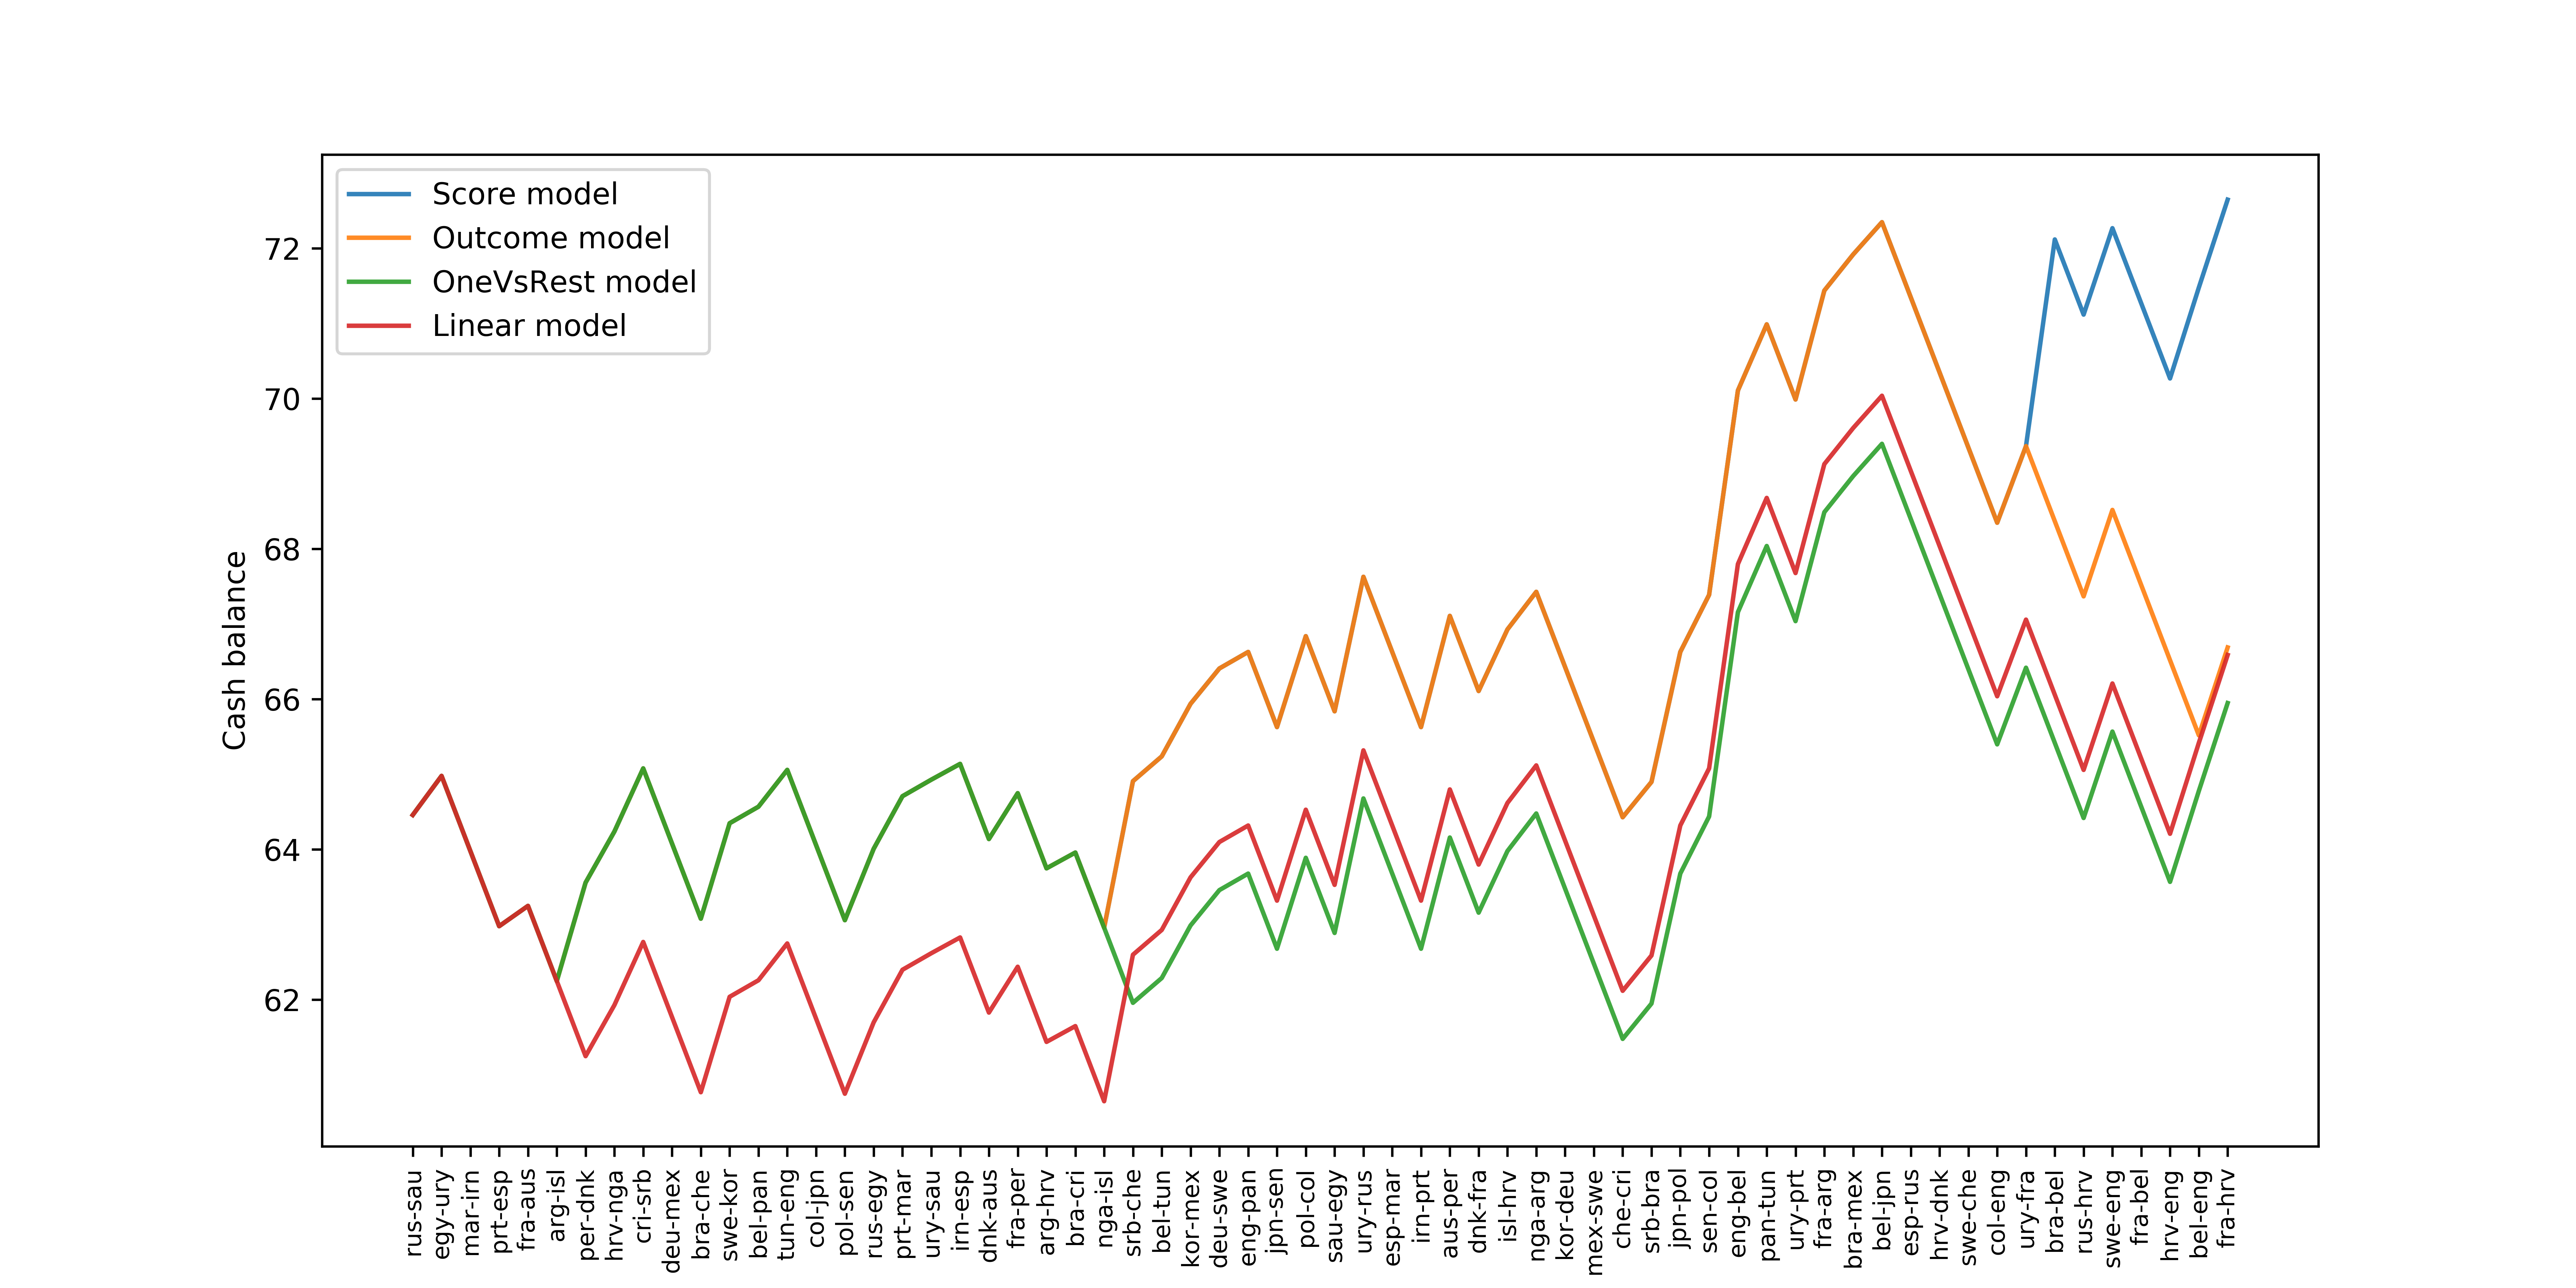
\includegraphics[width=0.7\textwidth]{img/match_level_2018_model_unit.png}
    \caption{Unit strategy's cash balance progression on World Cup 2018.}
    \label{fig:unit_model_comparison}
\end{figure}

\begin{figure}[H]
    \centering
    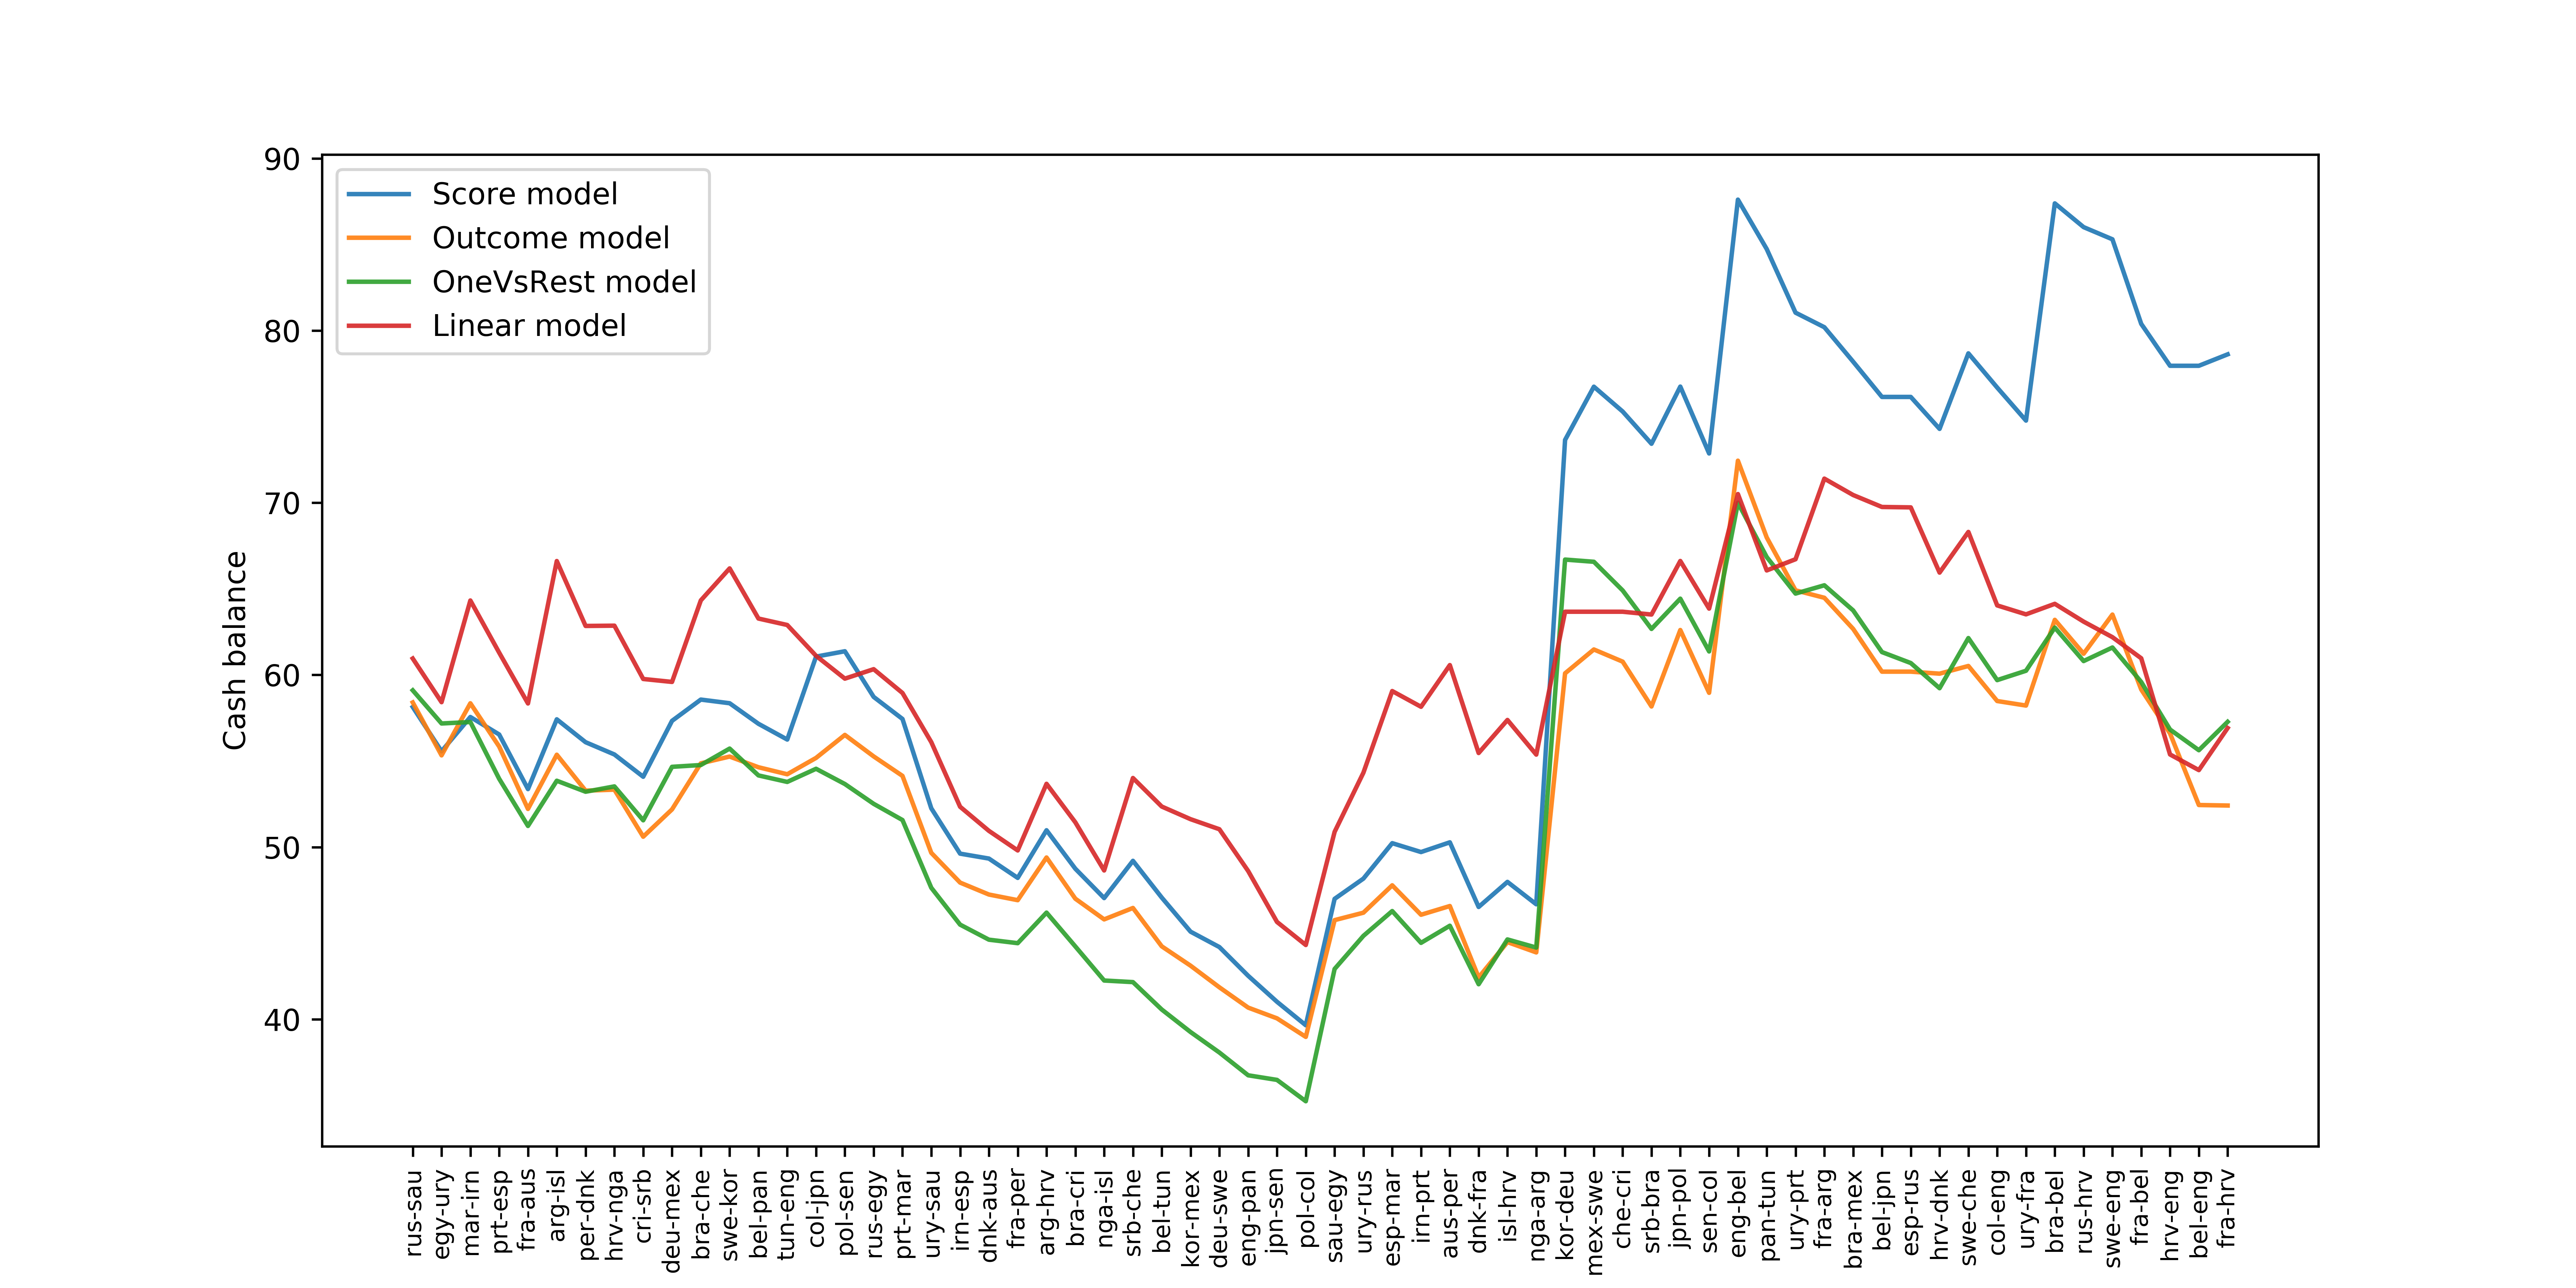
\includegraphics[width=0.7\textwidth]{img/match_level_2018_model_kelly.png}
    \caption{Kelly strategy's cash balance progression on World Cup 2018.}
    \label{fig:kelly_model_comparison}
\end{figure}

\begin{figure}[H]
    \centering
    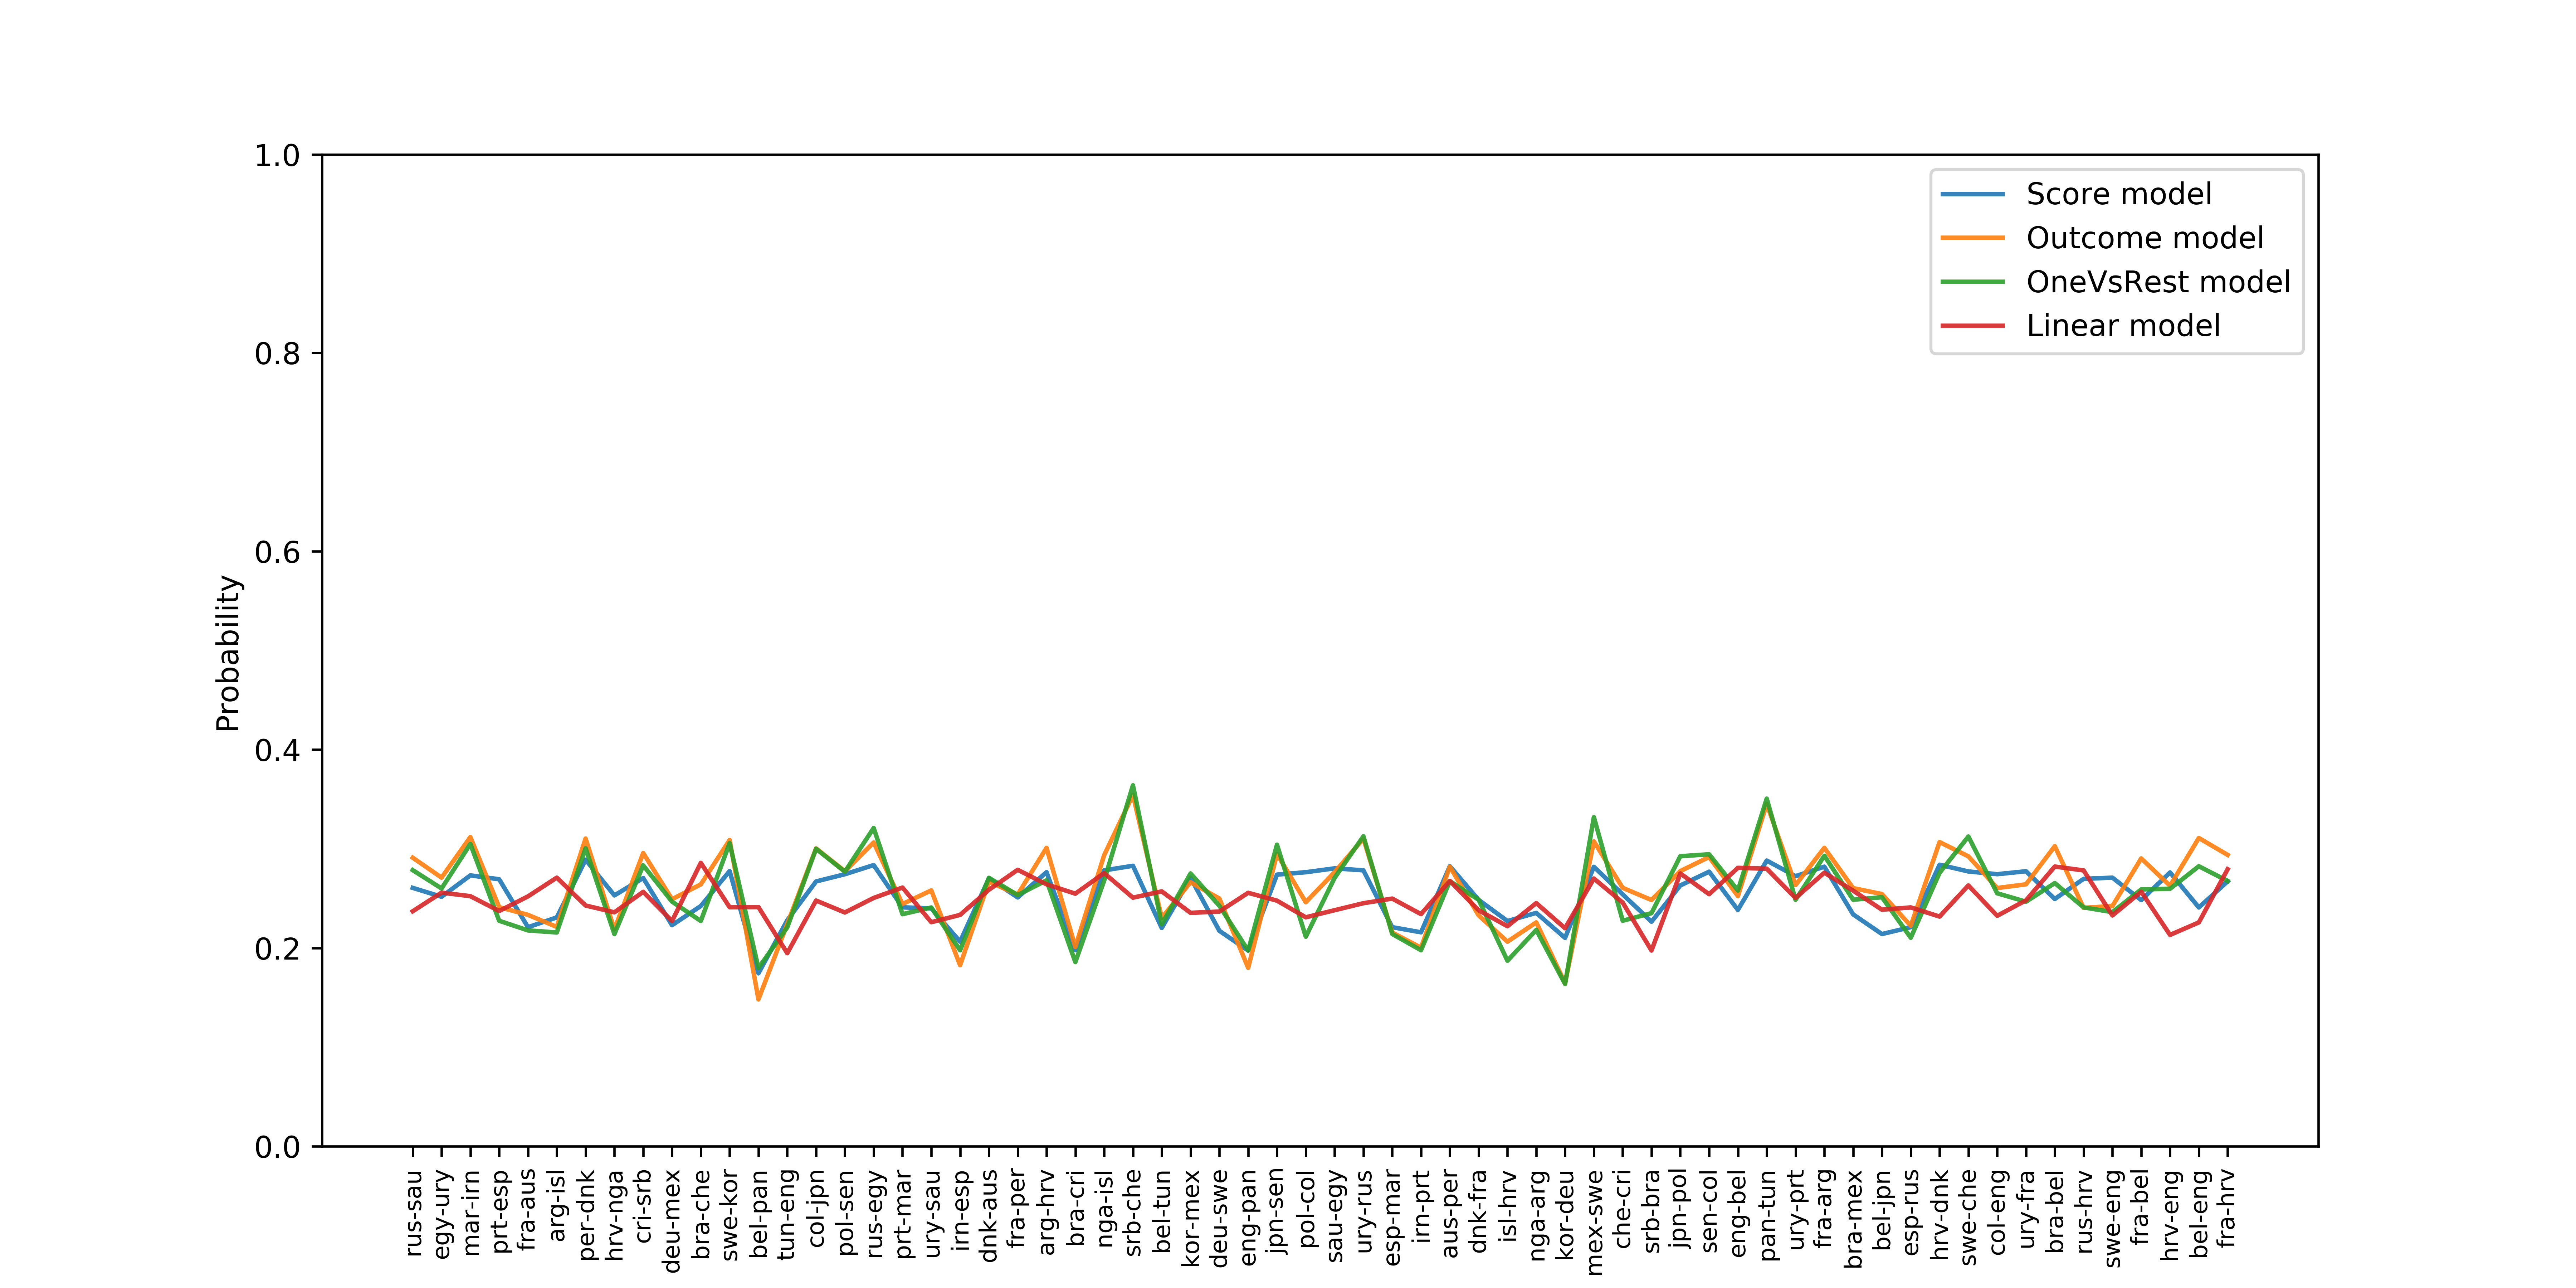
\includegraphics[width=0.7\textwidth]{img/match_level_2018_model_probability_draw_prob.png}
    \caption{Predicted probability of draw in the World Cup 2018.}
    \label{fig:draw_probability}
\end{figure}

\begin{figure}[H]
    \centering
    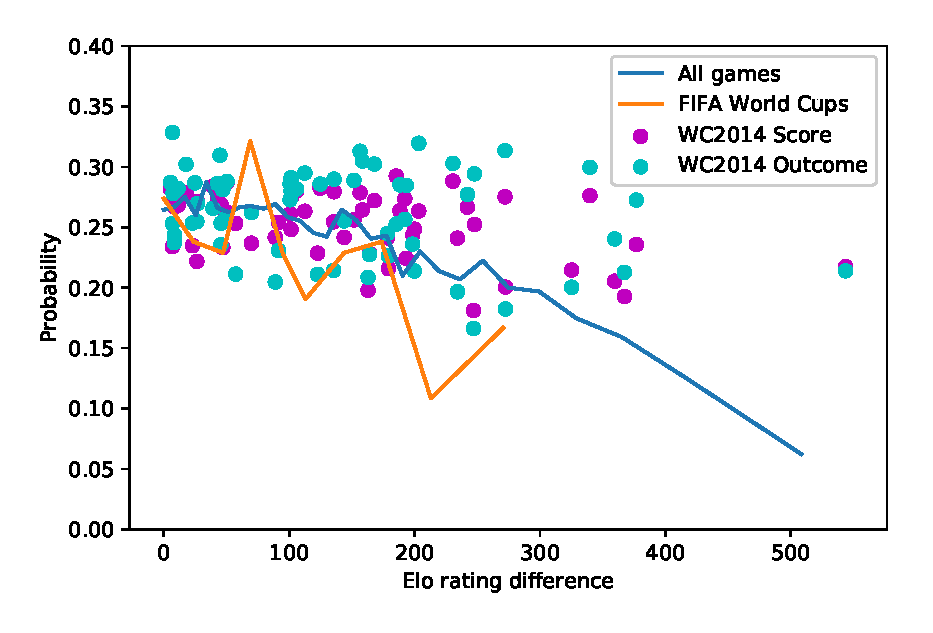
\includegraphics[width=0.7\textwidth]{img/draw_true_probability_wc.eps}
    \caption{Predicted probabilities vs. sample probability distribution. Sample probability distribution of draw is calculated from all international football games between dates 11/30/1872 - 06/04/2018. Dots are single probability estimates from \textit{Score model} and \textit{Outcome model} for matches in World Cup 2014.}
    \label{fig:draw_prob_dist}
\end{figure}

\section{Feature set comparison}
It's interesting that feature sets with fewer features can produce better predictions. How can less describe more? It's against common sense, right?

These problems are visible if the models' accuracy is compared. Being one of the most important metrics, it's still not the most important for the sophisticated betting strategies like kelly, which utilizes model's probability estimates. Log loss is a metric that can be used to compare probability distributions' accuracy. A smaller value indicates a more accurate estimate. When log loss is compared per tournament model trained with limited feature set can have lower log loss value than the same model that is trained using all of the features. But when the average performance from every tournament is considered training model with all features seems to output the lowest log loss score with \textit{Outcome model} and \textit{OVR model} and second lowest (only 0.0009 difference at highest) with \textit{Score model} and \textit{Linear model}. This indicates that even-though increasing accuracy might not benefit from using all features probability distribution prediction clearly benefits. Since football games often have low scores can last-minute surprises change the outcome of the match. The underdog can beat the favorite or at least square the game. This means that achieving high accuracy is hard, but fixing probabilities to match the true ones has more room to improve.

Feature importance can be calculated with Random Forest. These values can give insight on models reasoning. This data combined with optimal hyperparameters is one way to interpret the models since inspecting every single tree in the forest would be too cumbersome.

Segal \cite{segal2004machine} showed that noisy variable can lead to higher optimal value for minimum samples at leaf hyperparameter. With generic features models seem to prefer higher value for the hyperparameter \textit{minimum samples at leaf} as we can see from the table \ref{table:hyperparam_results}.  Figure \ref{fig:outcome_feature_importance_gf} lists feature importance for Outcome model trained with generic features. Difference between elo rating dominates the others, but just by looking at the plot it's impossible to say if any of the features could be considered to be just noise. Lower importance features like \textit{home\_goal} and \textit{away\_goal} seem to be in the middle tier when model is trained with all features. This higher importance compared to other features could mean that these features have predicting power.

With \textit{player features} difference between features is not that big. Feature importance is gradually decreasing feature by feature as we can see from the figure \ref{fig:outcome_feature_importance_pf}. Same features seem to rank high with player features as they would with all features.

\begin{table}
    \caption{Hyperparameter selection results for random forest models.}
    \begin{tabular}{| c  c| c| c| c|}
        \hline
        Model & Features & \# of predictors & Min samples at leaf & Max depth\\
        \hline
        Score & AF & $\sqrt{M}$ & 1 & 8 \\
         & GF & $\log_2{M}$ & 10 & 8 \\
         & PF & $\sqrt{M}$ & 5 & Na \\
         \hline
        Outcome & AF & $\sqrt{M}$ & 3 & 8 \\
         & GF & $\log_2{M}$ & 15 & 5 \\
         & PF & $\log_2{M}$ & 3 & 8 \\
        \hline
        OVR & AF home win & $\sqrt{M}$ & 3 & 5 \\
        OVR & AF draw & $\sqrt{M}$ & 5 & Na \\
        OVR & AF away win & $\sqrt{M}$ & 3 & 5 \\
        OVR & GF home win & $\sqrt{M}$ & 10 & 12 \\
        OVR & GF draw & $\log_2{M}$ & 15 & 8 \\
        OVR & GF away win & $\log_2{M}$ & 10 & 5 \\
        OVR & PF home win & $\log_2{M}$ & 3 & 5 \\
        OVR & PF draw & $\log_2{M}$ & 15 & 5 \\
        OVR & PF away win & $\log_2{M}$ & 5 & 8 \\
        \hline
    \end{tabular}
    \label{table:hyperparam_results}
\end{table}

\begin{figure}[H]
    \centering
    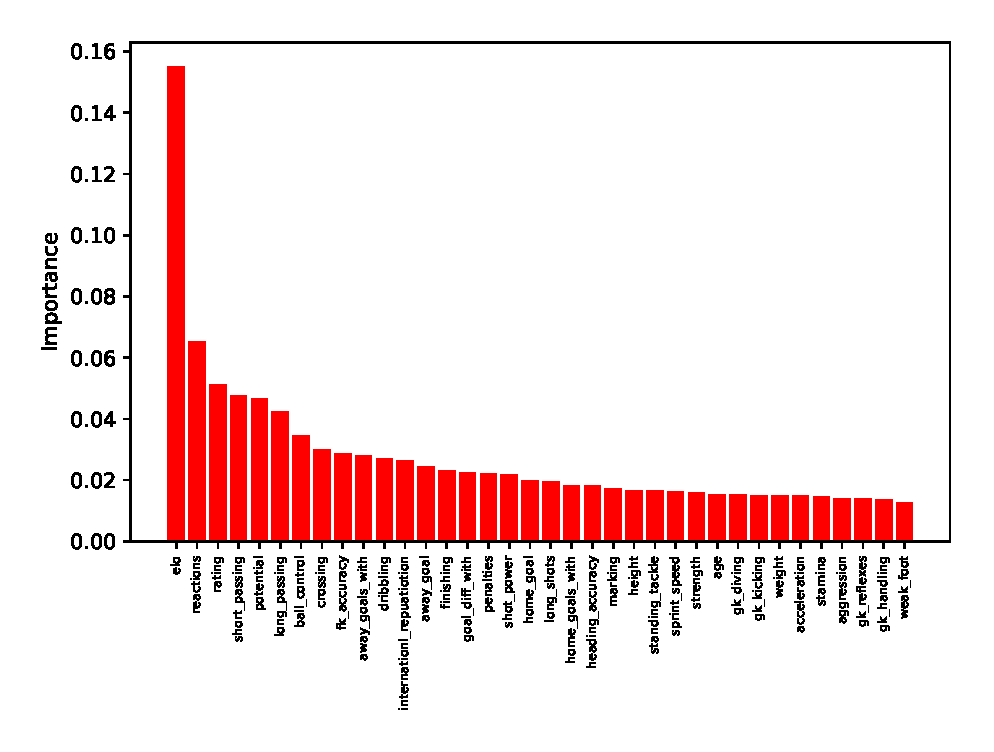
\includegraphics[width=0.7\textwidth]{img/match_level_2018_outcome_feature_importance_af_feature_importance.eps}
    \caption{Outcome model's feature importance with all features.}
    \label{fig:outcome_feature_importance_af}
\end{figure}

\begin{figure}[H]
    \centering
    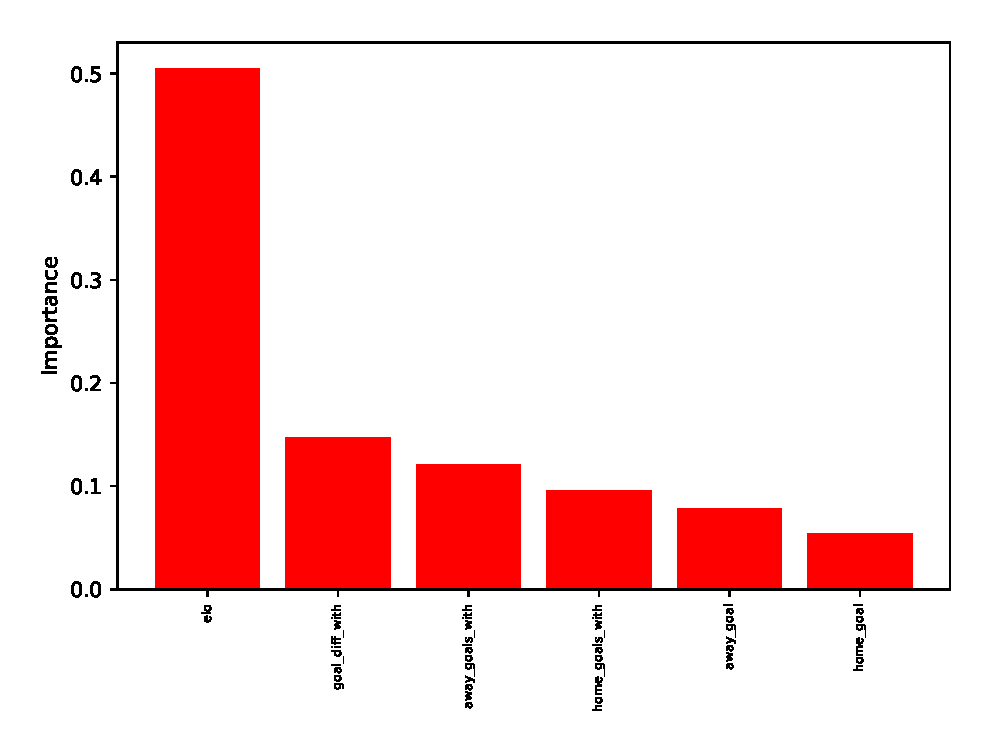
\includegraphics[width=0.7\textwidth]{img/match_level_2018_outcome_feature_importance_gf_feature_importance.eps}
    \caption{Outcome model's feature importance with generic features.}
    \label{fig:outcome_feature_importance_gf}
\end{figure}

\begin{figure}[H]
    \centering
    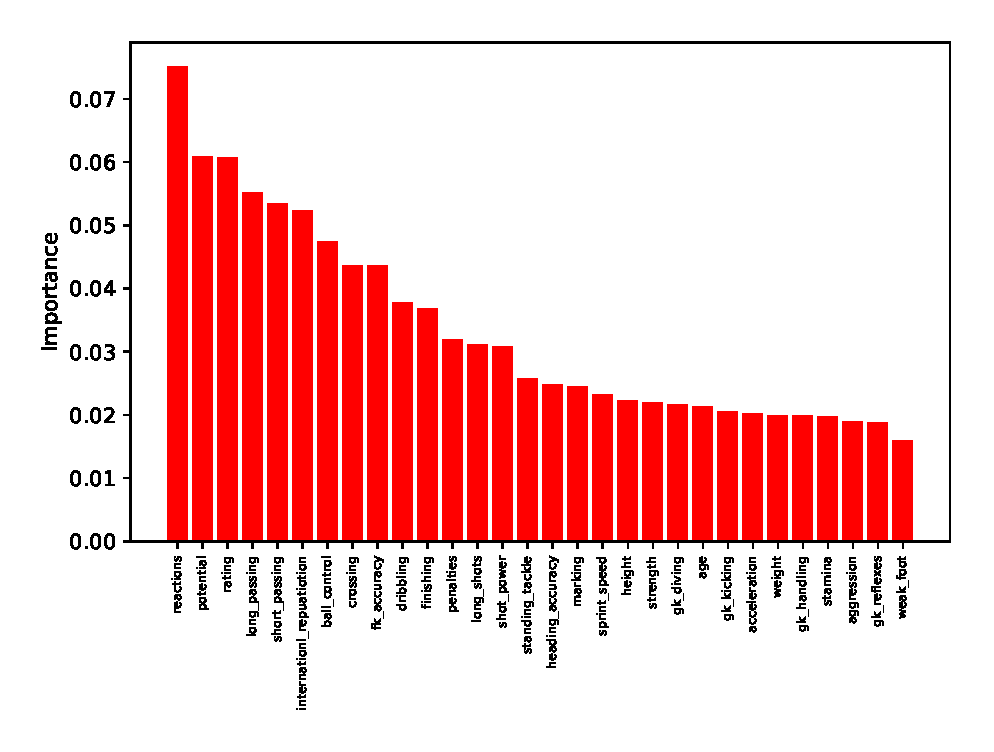
\includegraphics[width=0.7\textwidth]{img/match_level_2018_outcome_feature_importance_pf_feature_importance.eps}
    \caption{Outcome model's feature importance with player features.}
    \label{fig:outcome_feature_importance_pf}
\end{figure}

If some of the features are just noise, those features can be removed without harming the model's probability estimates. One way to do this is recursive feature elimination where one by one features are eliminated and models performance is measured for every elimination round. This test is done 100 times for every elimination round to guarantee that variation in the results won't cause features to be eliminated too early. I did the recursive feature elimination process the \textit{Outcome model}.

\section{Recursive feature elimination}
If some of the features are just noise, those features can be removed without harming the model's probability estimates. One way to do this is recursive feature elimination (RFE) where one by one features are eliminated and models performance is measured for every elimination round. The least important feature is eliminated each round. Accuracy and log loss are measured 100 times for each round to account for natural variance in the results. Feature elimination process is started again until there are no features left. Stored average accuracy and average log loss can be used to see how the model's performance evolved during RFE. All of the test were done with \textit{Outcome model}.

First test included default parameters for \textit{Outcome model}: 1000 for number of estimators, $\sqrt{M}$ for number of predictors, Na for maximum depth and one for minimum samples at leaf. From figure \ref{fig:def_avg_accu} we can see that after \textit{gk\_diving} accuracy starts to decrease slowly. If we compare this result to figure \ref{fig:def_avg_loss}
it's evident that the performance decreases after \textit{gk\_diving}. For comparison I run the same test with \textit{Outcome model} using optimal parameters used in all feature setup in the table \ref{table:outcomemodel}. Results are visible in the figures \ref{fig:optimal_avg_accu} and \ref{fig:optimal_avg_loss}. With this setup model performs better through out the whole RFE process. Also, model peaks the highest accuracy with only just four features. Improvement with this same feature set is not visible in the average log loss. The average log loss has a clear performance drop only when there is a single feature left.

To test model's performance with limited feature set I ran the World cup simulation for \textit{Outcome model} using features: \textit{away\_goals\_with\_home, finishing\_diff, height\_diff, crossing\_diff, potential\_diff, fk\_accuracy\_diff, home\_goal\_mean, away\_goal\_mean, ball\_control\_diff, long\_passing\_diff,  short\_passing\_diff, reactions\_diff, rating\_diff, elo\_diff}. I chose these features since they were the smallest feature set that was able to keep the performance with a model trained with default hyperparamaters. New optimal hyperparameters where grid searched for this feature set. These hyperparameters are listed in the table \ref{table:hyperparam_results_rfe} and World Cup simulation results are in the table \ref{table:outcomemodel_rfe}. Based on the results model's performance according to accuracy and log loss doesn't differ significantly from the model that was trained using all features.

Based on the progression of the average accuracy and the average log loss models do not perform better when features are removed from the original feature set. Eventually performance decreases but never increases during feature elimination. Most of the time results just have natural variance, which causes small changes. It seems that using every available feature doesn't harm random forest's performance, even though there is no guarantee that all of the features are useful. Also, RFE's suitability for this setup can be questioned. Stroble et al. concluded: "In particular, the selection of the first splitting variable involves only the marginal, univariate association between that predictor variable and the response, regardless of all other predictor variables. However, this search strategy leads to a variable selection pattern where a predictor variable that is per se only weakly or not at all associated with the response, but is highly correlated with another influential predictor variable, may appear equally well suited for splitting as the truly influential predictor variable." This can be problematic since removing one of the correlated predictors decreases impurity significantly and this effect is not as visible when the rest of the correlated predictors are removed. This leads to a situation where importance of a feature is measured incorrectly.
\begin{figure}[H]
    \centering
    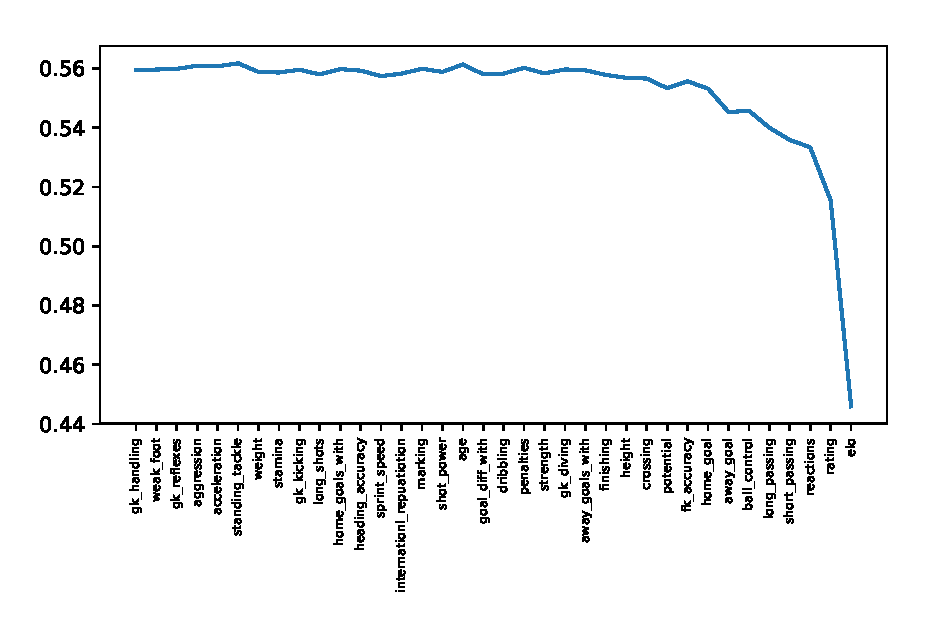
\includegraphics[width=0.7\textwidth]{img/default_avg_accuracy.eps}
    \caption{Mean accuracy for recursive feature elimination on outcome model with default parameters.}
    \label{fig:def_avg_accu}
\end{figure}

\begin{figure}[H]
    \centering
    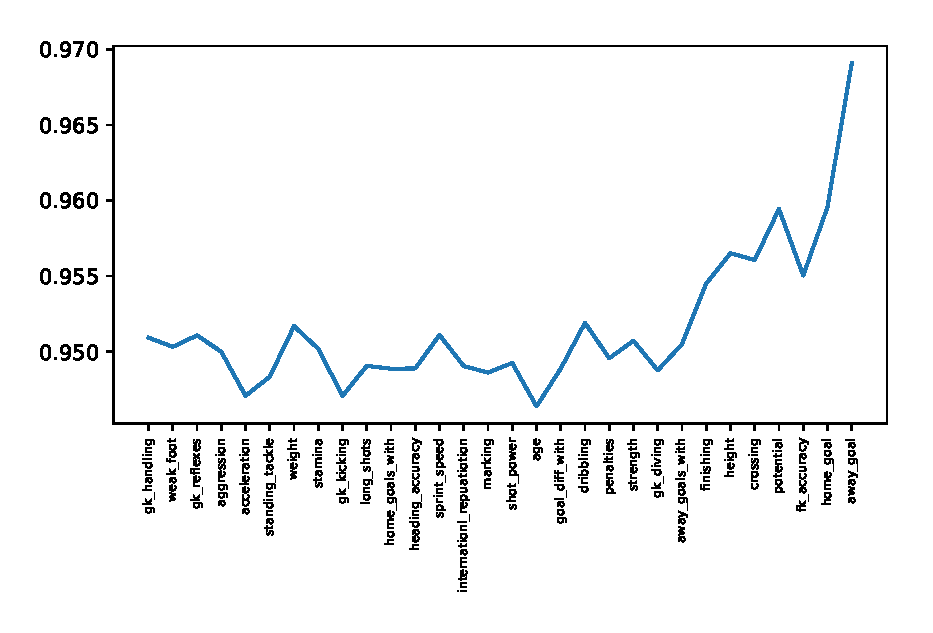
\includegraphics[width=0.7\textwidth]{img/default_avg_lloss.eps}
    \caption{Mean log loss for recursive feature elimination on outcome model with default parameters. Only features from first round to the 30th round are list to ensure figure's readability.}
    \label{fig:def_avg_loss}
\end{figure}

\begin{figure}[H]
    \centering
    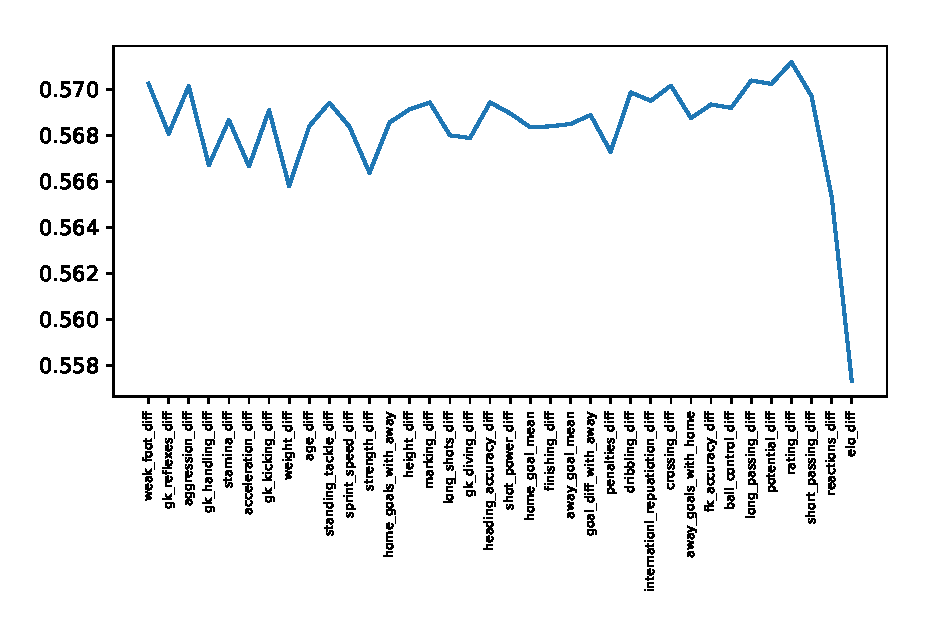
\includegraphics[width=0.7\textwidth]{img/optimal_avg_accuracy.eps}
    \caption{Mean accuracy for recursive feature elimination on outcome model with optimal parameters for all features setup in the table \ref{table:outcomemodel}.}
    \label{fig:optimal_avg_accu}
\end{figure}

\begin{figure}[H]
    \centering
    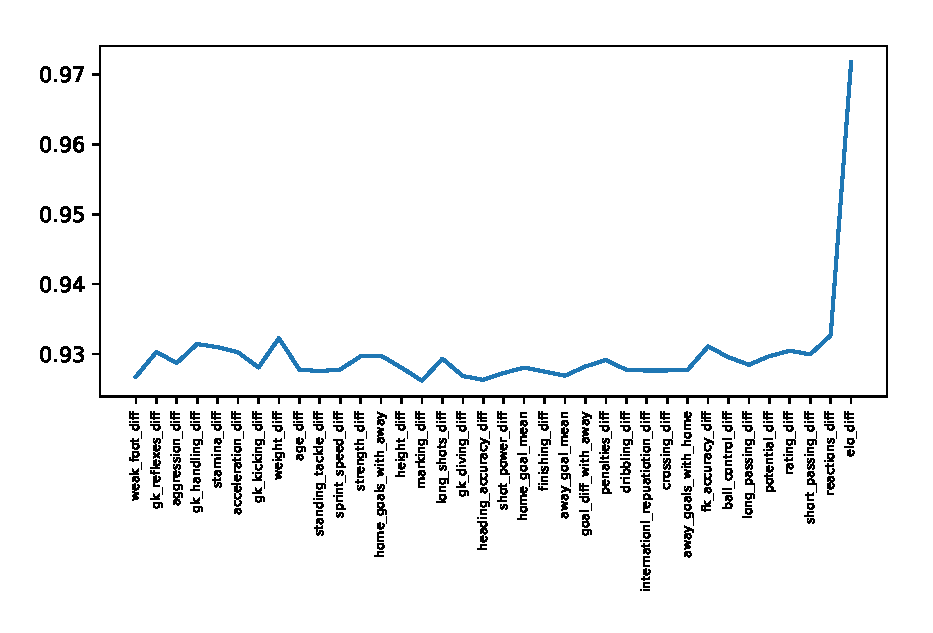
\includegraphics[width=0.7\textwidth]{img/optimal_avg_lloss.eps}
    \caption{Mean log loss for recursive feature elimination on outcome model with optimal parameters for all features setup in the table \ref{table:outcomemodel}.}
    \label{fig:optimal_avg_loss}
\end{figure}

\begin{table}
    \caption{Results for Outcome model with limited features from RFE.}
    \begin{tabular}{| c | c| c| c|c|}
        \hline
        Metric& \textbf{WC 2018} & \textbf{WC 2014} & \textbf{WC 2010} & Mean\\
        \hline
        Accuracy  & 52.97\% $\pm$ 2.36 & 59.69\% $\pm$ 2.3 & 56.09\% $\pm$ 2.47& 56.25 \\
        Log Loss & 0.9953 $\pm$ 0.0087 & 0.9282 $\pm$ 0.0061 & 0.9743 $\pm$ 0.0069& 0.9659 \\
        Unit profit  & -1.79\% $\pm$ 6.16 & 14.12\% $\pm$ 6.02 & 8.82\% $\pm$ 7.47& 7.05 \\
        Kelly profit  & -37.19\% $\pm$ 11.43 & 61.45\% $\pm$ 15.42 & 77.87\% $\pm$ 12.98& 34.04 \\
 \hline
    \end{tabular}
    \label{table:outcomemodel_rfe}
\end{table}

\begin{table}
    \caption{Optimal hyperparameters for Outcome model trained with RFE feature set.}
    \begin{tabular}{| c | c| c| c|}
        \hline
         \# of predictors & Min samples at leaf & Max depth\\
        \hline
         $\sqrt{M}$ & 10 & Na \\
        \hline
    \end{tabular}
    \label{table:hyperparam_results_rfe}
\end{table}


\subsection{Match-level betting activity - what drives the profits?}
As it's mentioned many times unit strategy can be considered as a dummy strategy; one unit for the predicted winner. Kelly strategy instead is more sophisticated and deserves a deeper analysis. With the requirements 1) profitable in every tournament, and 2) best average profits has \textit{Score model} trained with all features performed the best with kelly strategy. For this reason \textit{Score model} is used to get the results for the following figures.

The most successful tournament for \textit{Score model} was World Cup 2018. It achieved, on average, 35.59\% profit. In comparison profit from World Cup 2014 was only 12.37\%. By the numbers performance in World Cup 2018 was definitely better, but what happened with match-level betting? When we compare both of the tournaments side by side in the figures \ref{fig:net_win_cost_2018} and \ref{fig:net_win_cost_2014} it's clear that a single successful bet dominates the profit in World Cup 2018. Don't get confused by the difference in the scale of y-axis. Total bets per match are not that different between the tournaments. Only betting frequency differs - there are more games in World Cup 2014 without any bets. With World Cup 2018 winnings are more rare, but the size is bigger. These anomalies in odds are certainly important and this strategy is able to utilize them properly. Without three biggest winnings this strategy would achieve negative profits for sure. With World Cup 2014 strategy wins more often, but winning as not as big as they are in World Cup 2018. This would be ideal as well for the World Cup 2018, but it's harder to achieve. When winnings are more frequent predicted probabilities need to be closer to the true ones than the implied probabilities from the betting market are. Based on the limited amount of evidence, smaller but more frequent winnings and sparser betting activity, it seems that the probability estimates for World Cup 2014 were better than the implied ones based on the market. Where as in World Cup 2018 profitability was based on the strategy's ability to gain from few favourable odds. The latter might be extremely hard to keep profitable in the long run unless betting market's dynamics create opportunities often enough. Model's bias towards higher probability of a draw compared to market's when difference between teams' elo rating is relatively high stands out in both of the tournaments. This harms the strategy's performance.

\begin{figure}[H]
    \centering
    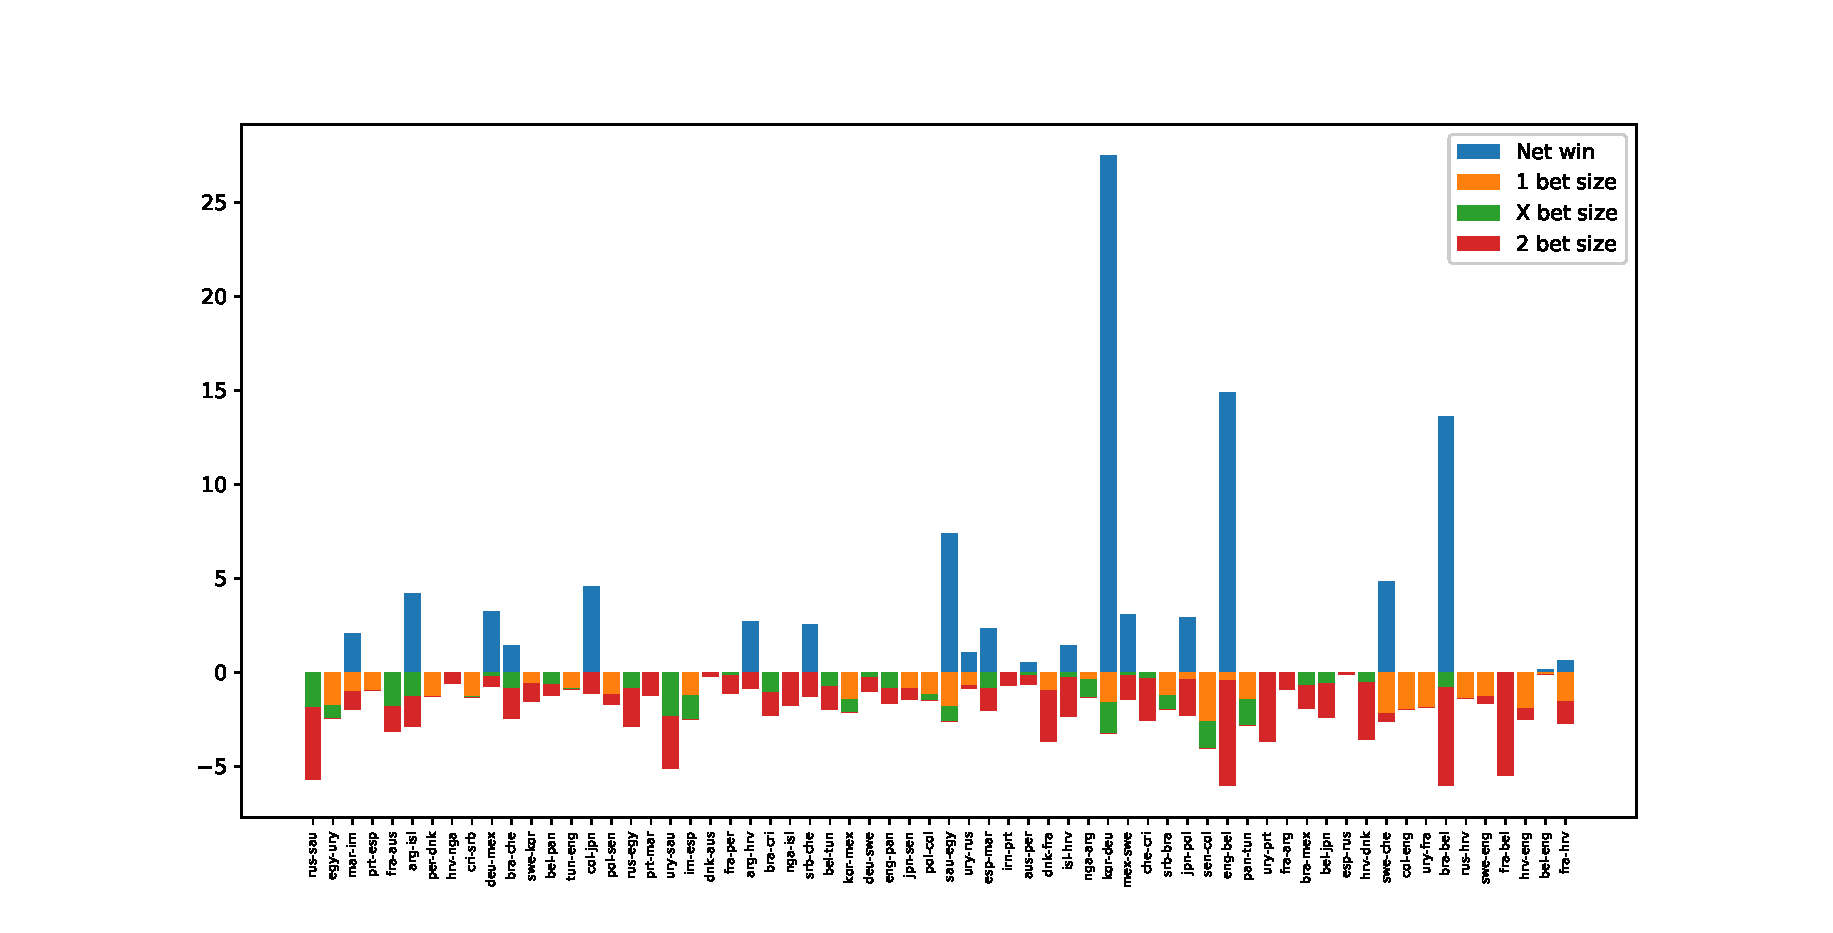
\includegraphics[width=0.7\textwidth]{img/match_level_2018_score_win_cost_.eps}
    \caption{Net winnings and betting costs per label for Score model in World Cup 2018.}
    \label{fig:net_win_cost_2018}
\end{figure}

\begin{figure}[H]
    \centering
    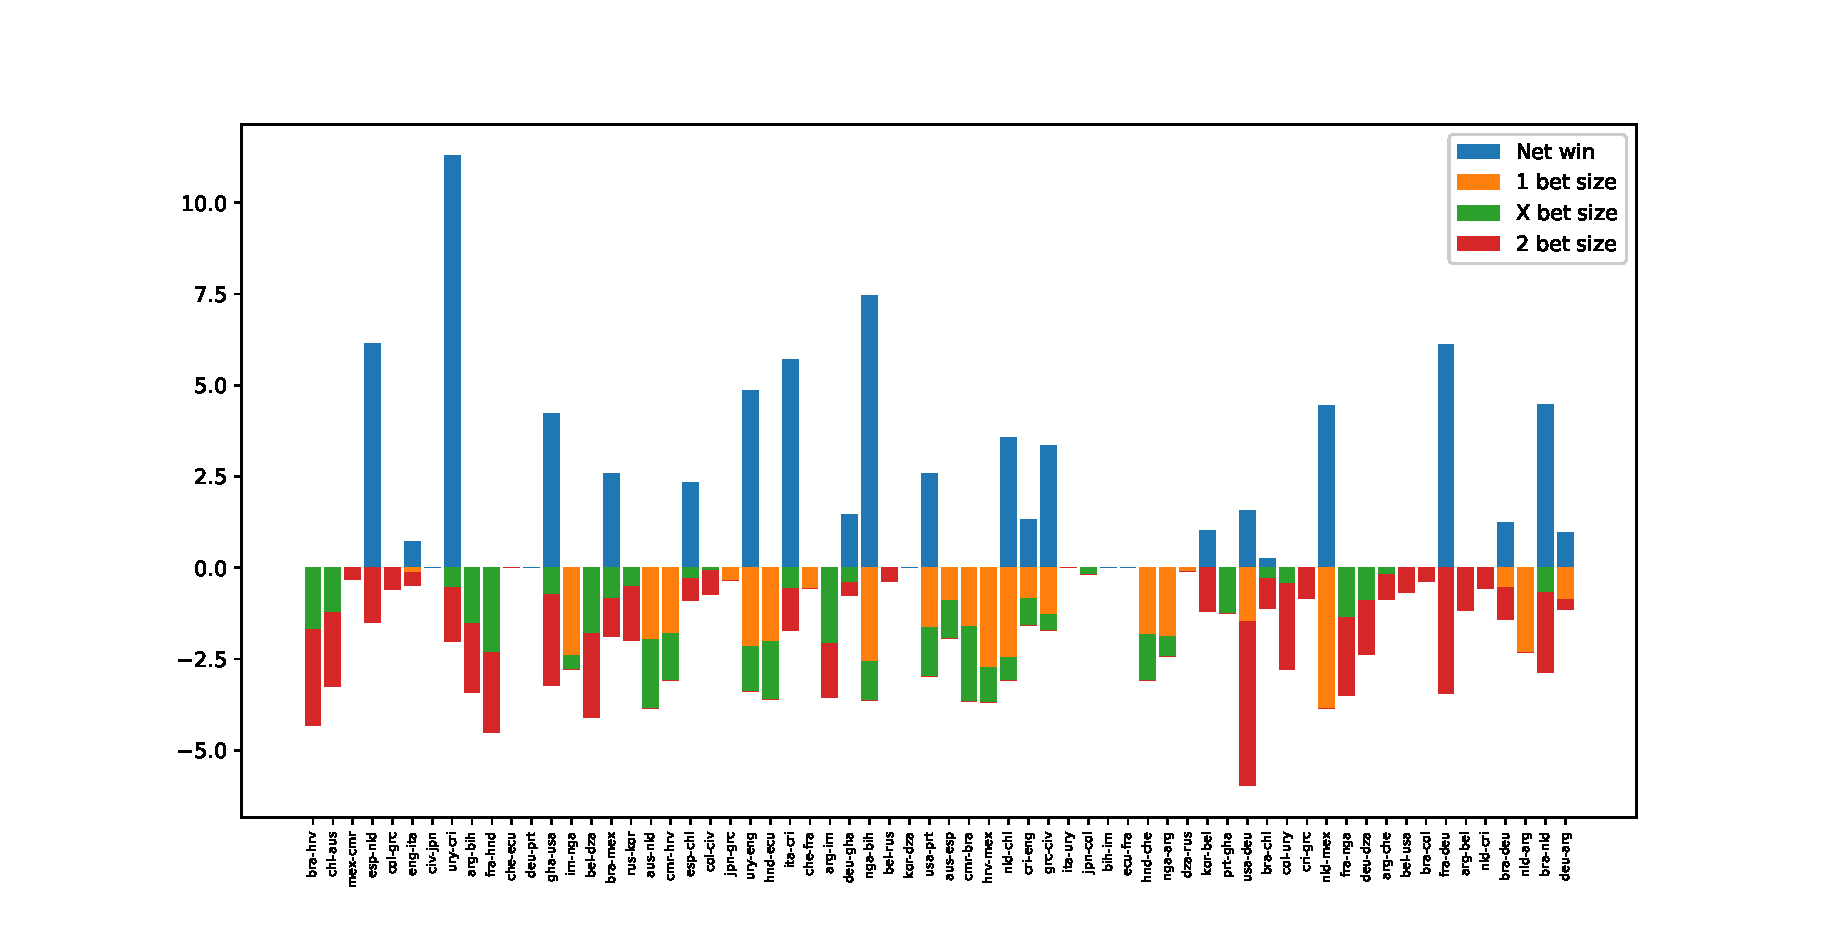
\includegraphics[width=0.7\textwidth]{img/match_level_2014_score_win_cost_.eps}
    \caption{Net winnings and betting costs per label for Score model trained with all features in World Cup 2014.}
    \label{fig:net_win_cost_2014}
\end{figure}